\documentclass{beamer}

\usetheme{Madrid}
\usecolortheme{seahorse}

\title{Introduzione ai Sistemi Operativi}
\subtitle{Fondamenti e Architettura}
\author{Prof. Fedeli Massimo - Corso ITS – Fabbrica Digitale}
\date{Parte 1}

\begin{document}
	
	\frame{\titlepage}
	
	%------------------------------------------------
	
	%------------------------------------------------
	\begin{frame}
		\frametitle{Cos'è un Sistema Operativo}
		
		Un Sistema Operativo (SO) è:
		
		\begin{itemize}
			\item Un insieme di \textbf{programmi} che gestisce le \textbf{risorse di un computer}
			\item Un intermediario tra \textbf{utente} e \textbf{hardware}
			\item Un ambiente di sviluppo ed esecuzione per le \textbf{applicazioni}
		\end{itemize}
		\vspace*{0.5 cm}
		\textbf{Cosa sono le risorse del computer?}
		
		Le risorse sono tutti i componenti hardware e software necessari
		all'esecuzione dei programmi.
		
		\begin{itemize}
			\item \textbf{CPU}: esegue le istruzioni dei programmi
			\item \textbf{Memoria RAM}: contiene dati e programmi in esecuzione
			\item \textbf{Memoria secondaria}: dischi SSD/HDD dove sono memorizzati i file
			\item \textbf{Dispositivi di I/O}: tastiera, mouse, stampante, rete, ecc.
		\end{itemize}
	
		
	\end{frame}
	
	
	\begin{frame}
				\frametitle{Cos'è un Sistema Operativo}
		Il sistema operativo decide \textbf{come e quando assegnare queste risorse}
ai programmi in esecuzione.

\textbf{Esempi di sistemi operativi}

\begin{itemize}
	\item Linux
	\item Windows
	\item macOS
	\item Android
\end{itemize}
	\end{frame}
	%------------------------------------------------
	
	\begin{frame}
		\frametitle{Ruolo del Sistema Operativo}
		
		Il sistema operativo:
		
		\begin{itemize}
			\item controlla la CPU
			\item gestisce la memoria
			\item gestisce i dispositivi di input/output
			\item gestisce file e dati
		\end{itemize}
		
	\end{frame}
	
	%------------------------------------------------
	
	\begin{frame}
		\frametitle{Struttura di un Sistema di Calcolo}
		
		\begin{center}
			
			Utenti
			
			$\downarrow$
			
			Applicazioni
			
			$\downarrow$
			
			Sistema Operativo
			
			$\downarrow$
			
			Hardware
			
		\end{center}

		
		\textbf{Il concetto di astrazione}
		
		Il sistema operativo fornisce un \textbf{livello di astrazione} sopra l'hardware,
		cioè nasconde la complessità dei componenti fisici del computer e
		presenta agli utenti e ai programmi un'interfaccia più semplice da usare.
	
		

		
	\end{frame}


\begin{frame}
	\frametitle{Titolo della slide}
	
	\begin{center}
		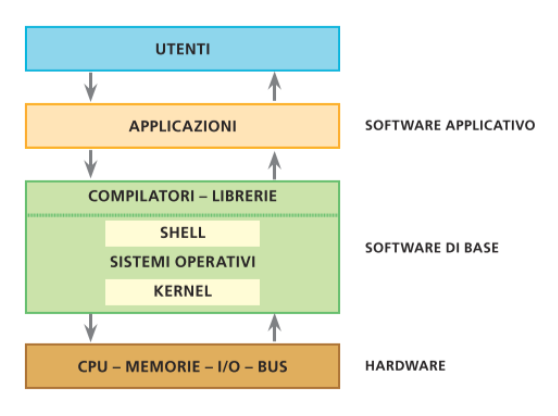
\includegraphics[width=0.8\textwidth]{astrazione.png}
	\end{center}
	
\end{frame}
	
		\begin{frame}
		\frametitle{Struttura di un Sistema di Calcolo}
	
		\textbf{Esempi di astrazione}
		
		\begin{itemize}
			\item \textbf{File}: i dati su disco vengono gestiti come file e cartelle,
			senza preoccuparsi dei settori fisici del disco.
			\item \textbf{Processi}: un programma in esecuzione viene visto come un
			processo, senza gestire direttamente CPU e registri.
			\item \textbf{Memoria virtuale}: ogni programma ha l'illusione di avere
			a disposizione tutta la memoria del sistema.
			\item \textbf{Dispositivi}: tastiere, dischi o stampanti sono accessibili
			tramite comandi standard, indipendentemente dall'hardware reale.
		\end{itemize}
		
		
		Grazie all'astrazione, i programmatori possono sviluppare software
		senza conoscere nei dettagli l'hardware della macchina.
		
	\end{frame}

	\begin{frame}
		\frametitle{Risorse gestite dal Sistema Operativo}
		
		\textbf{Principali risorse}:
		
		\begin{itemize}
			\item CPU
			\item Memoria RAM
			\item Memoria secondaria (dischi)
			\item Dispositivi di I/O
			\item Rete
		\end{itemize}
		
		Il SO decide come assegnare queste risorse ai programmi.
		
	\end{frame}
	
	%------------------------------------------------
	
\begin{frame}
	\frametitle{Obiettivi principali di un Sistema Operativo}
	
	Un sistema operativo deve garantire diversi obiettivi fondamentali
	per permettere al sistema di funzionare in modo efficiente e sicuro.
	
	\begin{itemize}
		
		\item \textbf{Efficienza nell'uso delle risorse} \\
		Il sistema operativo deve utilizzare al meglio le risorse disponibili
		(CPU, memoria, disco e dispositivi di I/O), evitando sprechi e
		riducendo i tempi di inattività del sistema.
		
		\item \textbf{Sicurezza} \\
		Il sistema operativo deve proteggere il sistema e i dati da accessi
		non autorizzati, garantendo meccanismi di autenticazione, permessi
		di accesso e isolamento tra processi e utenti.
		
		\item \textbf{Affidabilità} \\
		Il sistema deve continuare a funzionare correttamente anche in
		presenza di errori hardware o software, evitando crash e perdita
		di dati.
		
		\item \textbf{Condivisione delle risorse} \\
		In sistemi multiutente o multiprogrammati più programmi devono
		poter utilizzare le stesse risorse (CPU, memoria, periferiche)
		senza interferire tra loro.
		
		\item \textbf{Facilità d'uso} \\
		Il sistema operativo deve fornire interfacce semplici e intuitive,
		come la shell o l'interfaccia grafica, che permettono agli utenti
		di utilizzare il computer senza conoscere i dettagli dell'hardware.
		
	\end{itemize}
	
\end{frame}
	
	
	\begin{frame}
		\frametitle{Esempi pratici degli obiettivi di un Sistema Operativo}
		
	
		\begin{itemize}
			
			\item \textbf{Efficienza} \\
			In un computer moderno è possibile eseguire contemporaneamente
			browser, editor di testo e musica. Il sistema operativo assegna
			dinamicamente la CPU e la memoria a ciascun programma.
			
			\item \textbf{Sicurezza} \\
			In Linux o Windows ogni utente ha un proprio account e permessi
			di accesso ai file. Un utente normale non può modificare file
			di sistema senza privilegi di amministratore.
			
			\item \textbf{Affidabilità} \\
			Se un'applicazione si blocca (ad esempio un browser), il sistema
			operativo può terminare il processo senza bloccare tutto il sistema.
			
			\item \textbf{Condivisione delle risorse} \\
			Più programmi possono utilizzare contemporaneamente la stessa
			stampante o la stessa connessione di rete.
			
			\item \textbf{Facilità d'uso} \\
			Le interfacce grafiche (Windows, macOS, GNOME, KDE) permettono
			di gestire file e programmi tramite finestre, icone e menu.
			
		\end{itemize}
		
	\end{frame}
	%------------------------------------------------
	
	\begin{frame}
		\frametitle{Il  modello ad anelli}
		Nel modello a ring i programmi che compongono il sistema operativo prendono il nome di moduli e sono raggruppati in anelli (ring), annidati dal più interno (hardware) fino al più esterno (shell).
		\begin{center}
			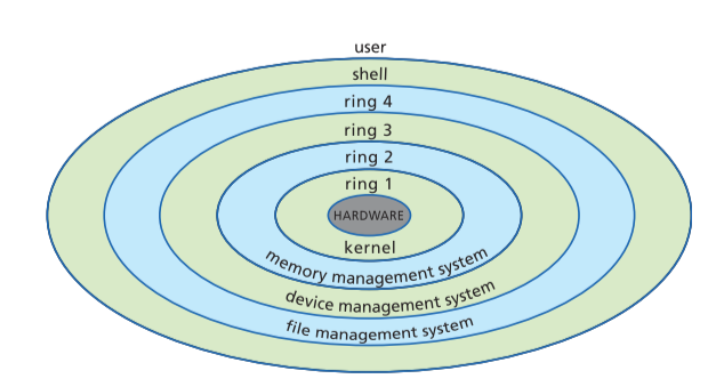
\includegraphics[width=0.8\textwidth]{cipolla.png}
		\end{center}
		
	\end{frame}
	
	\begin{frame}
		\frametitle{Il modello ad anelli}
		
		Il modello a ring, detto anche a buccia di cipolla, rappresenta
		il sistema operativo come costituito dai seguenti 4 ring:
		
		\begin{itemize}
			\item kernel (nucleo);
			\item memory management system (sistema di gestione della memoria);
			\item device management system (sistema di gestione delle periferiche);
			\item file management system (sistema di gestione delle informazioni).
		\end{itemize}
		
		Ogni anello rappresenta una macchina astratta diversa, costituita
		dai moduli software di quell'anello e dagli anelli a esso interni,
		fino all'hardware.
		
	\end{frame}
	
	
	\begin{frame}
		\frametitle{Evoluzione dei Sistemi Operativi}
		
		Le principali fasi storiche:
		
		\begin{enumerate}
			\item Prima generazione (anni 50)
			\item Sistemi batch
			\item Multiprogrammazione
			\item Time sharing
			\item Sistemi moderni
		\end{enumerate}
		
	\end{frame}
	
	%------------------------------------------------
	
	\begin{frame}
		\frametitle{Prima generazione (anni 50)}
		
		Caratteristiche:
		
		\begin{itemize}
			\item Programmazione in linguaggio macchina
			\item Input tramite schede perforate
			\item Nessun sistema operativo
		\end{itemize}
		
		Ogni programma controllava direttamente l'hardware.
		
	\end{frame}
	
	%------------------------------------------------
\begin{frame}
	\frametitle{Sistemi Batch}
	
	\textbf{Batch} significa letteralmente \textit{lotto} o \textit{gruppo}.
	
	Nei primi sistemi informatici i programmi venivano raccolti
	in gruppi (batch) ed eseguiti automaticamente uno dopo l'altro.
	
	
	\textbf{Come funzionava}
	
	\begin{itemize}
		
		\item Gli utenti preparavano i propri programmi (detti \textbf{job}).
		
		\item I programmi venivano consegnati all'operatore del computer,
		spesso tramite \textbf{schede perforate} o nastri magnetici.
		
		\item L'operatore caricava un \textbf{lotto di job} nel sistema.
		
		\item Il sistema operativo eseguiva i job \textbf{in sequenza},
		senza alcuna interazione con l'utente.
		
	\end{itemize}
	
	\textbf{Caratteristiche principali}
	
	\begin{itemize}
		
		\item Nessuna interazione diretta con il computer
		\item Esecuzione automatica dei programmi
		\item Ogni job iniziava solo dopo la terminazione del precedente
		
	\end{itemize}
	
\end{frame}
	
	%------------------------------------------------
	
	\begin{frame}[fragile]
		\frametitle{Esempio di Job Batch}
		
		\begin{verbatim}
JOB BEGIN
$compile
$load
$run
JOB END
\end{verbatim}
		
		Il sistema operativo eseguiva automaticamente i job.
		
	\end{frame}
	
	%------------------------------------------------
	
	\begin{frame}
		\frametitle{Limiti dei sistemi Batch}
		
		Problemi principali:
		
		\begin{itemize}
			\item CPU spesso inattiva durante I/O
			\item nessuna interazione con l'utente
			\item esecuzione sequenziale dei job
		\end{itemize}
		
	\end{frame}
	
	%------------------------------------------------

	
	%------------------------------------------------
\begin{frame}
	\frametitle{Multiprogrammazione}
	
	Nei sistemi batch semplici la \textbf{CPU rimaneva spesso inattiva}
	quando un programma era in attesa di operazioni di I/O
	(lettura da disco, stampa, accesso a dispositivi).
	
	
	\textbf{Idea della multiprogrammazione}
	
	\begin{itemize}
		
		\item Più programmi (\textbf{job}) vengono caricati
		contemporaneamente nella memoria principale.
		
		\item Il sistema operativo mantiene un insieme di programmi
		pronti per l'esecuzione.
		
		\item Quando un programma deve attendere un'operazione di I/O,
		la CPU viene assegnata ad un altro programma.
		
	\end{itemize}
	
	
	\textbf{Obiettivo}
	
	\begin{itemize}
		
		\item Ridurre i tempi di inattività della CPU
		\item Aumentare l'utilizzo delle risorse del sistema
		\item Migliorare le prestazioni complessive del computer
		
	\end{itemize}
	
\end{frame}
	 
	 
	 \begin{frame}
	 	\frametitle{La monoprogrammazione}
	 	\begin{center}
	 		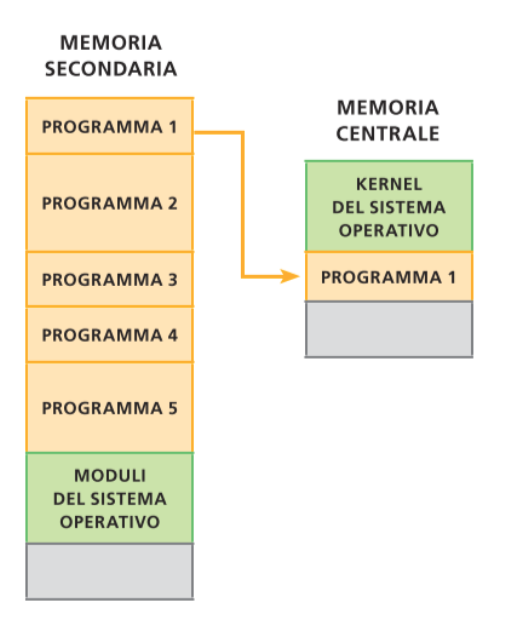
\includegraphics[width=0.5\textwidth]{monoprogrammazione.png}
	 	\end{center}
	 	
	 \end{frame}
	 
	 	 \begin{frame}
	 	\frametitle{La multi programmazione}
	 	\begin{center}
	 		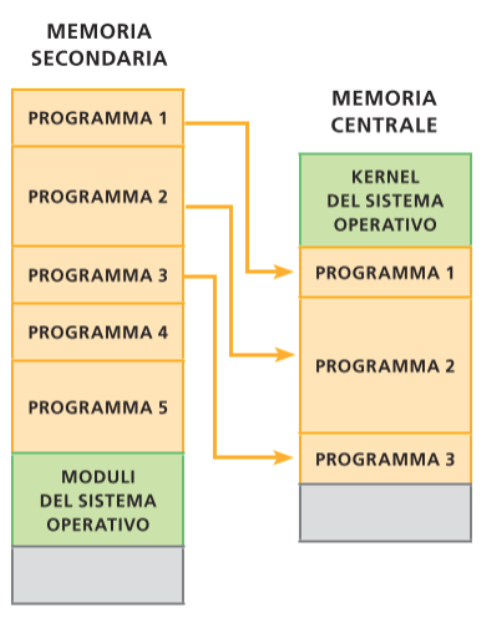
\includegraphics[width=0.5\textwidth]{multiprogrammazione.png}
	 	\end{center}
	 	
	 \end{frame}
	 
\begin{frame}
	\frametitle{Multiprogrammazione: utilizzo della CPU}
	
	Nei sistemi multiprogrammati più programmi condividono la CPU.
	
	Quando un programma è in attesa di un'operazione di I/O,
	il sistema operativo assegna la CPU ad un altro programma.

	
	\textbf{Esempio di utilizzo della CPU nel tempo}
	
	\begin{center}
		\begin{semiverbatim}
			tempo \(\rightarrow\)
			
			Job 1 : [CPU][CPU][ I/O  ][ I/O  ][ I/O  ][CPU][CPU]
			
			Job 2 :           [CPU][CPU][CPU][ I/O  ][ I/O  ]
			
			Job 3 :                         [CPU][CPU][CPU][CPU]
		\end{semiverbatim}
	\end{center}
	
	
	\textbf{Risultato}
	
	\begin{itemize}
		\item la CPU rimane attiva per la maggior parte del tempo
		\item più programmi avanzano nella loro esecuzione
		\item il sistema utilizza meglio le risorse disponibili
	\end{itemize}
	
\end{frame}
	%------------------------------------------------
	
	\begin{frame}
		\frametitle{Scheduling}
		
		Lo \textbf{scheduling} decide:
		
		\begin{itemize}
			\item quale processo usare la CPU
			\item quando cambiare processo
		\end{itemize}
		
		Tipi principali:
		
		\begin{itemize}
			\item\textbf{Long term }scheduling
			\item \textbf{Short term }scheduling
		\end{itemize}
		
	\end{frame}
		 \begin{frame}
		\frametitle{Scheduling}
		\begin{center}
			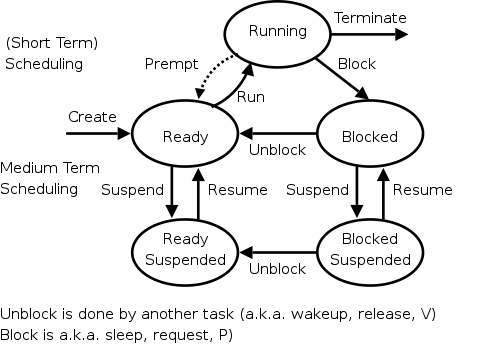
\includegraphics[width=0.7\textwidth]{longshortscheduling.png}
		\end{center}
		
	\end{frame}
	%------------------------------------------------
	
	\begin{frame}
		\frametitle{Long Term vs Short Term Scheduling}
	
		\textbf{Short Term Scheduling (CPU Scheduler)}
		\begin{itemize}
			\item Seleziona il processo da eseguire sulla CPU
			\item Gestisce la coda dei processi \textit{ready}
			\item Agisce con alta frequenza
			\item Transizione: \textit{ready} $\rightarrow$ \textit{running}
		\end{itemize}
		
	\end{frame}
	
\begin{frame}
	\frametitle{Time Sharing}
	
	Il \textbf{time sharing} è un'evoluzione dei sistemi multiprogrammati
	che introduce l'\textbf{interazione diretta tra utente e computer}.
	
	Nei primi sistemi informatici l'utente non interagiva direttamente
	con il computer: i programmi venivano eseguiti in modalità batch.
	
	Con il time sharing diventa possibile lavorare
	\textbf{interattivamente} con il sistema.
	
	\textbf{Caratteristiche principali}
	
	\begin{itemize}
		\item più utenti possono utilizzare il sistema contemporaneamente
		\item ogni utente può eseguire uno o più programmi
		\item il sistema operativo gestisce la condivisione delle risorse
	\end{itemize}
	
\end{frame}

		 \begin{frame}
	\frametitle{Scheduling}
	\begin{center}
		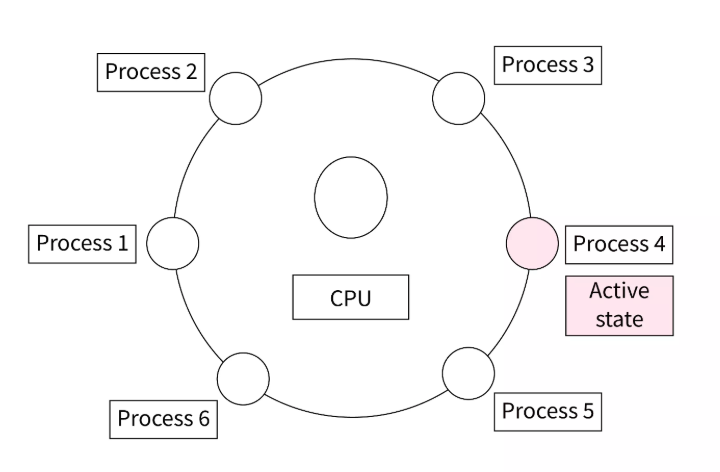
\includegraphics[width=0.7\textwidth]{timesharing.png}
	\end{center}
	
\end{frame}


\begin{frame}
\frametitle{Divisione della CPU nel Time Sharing}

Per permettere a più utenti di utilizzare il sistema,
la CPU viene suddivisa in piccoli intervalli di tempo.

Questi intervalli sono chiamati:

\begin{center}
	\textbf{time slice} oppure \textbf{quanto di tempo}
\end{center}

Il sistema operativo assegna la CPU ad un processo
per un breve intervallo di tempo.

Quando il tempo termina:

\begin{itemize}
	\item il sistema operativo interrompe il processo corrente
	\item salva il suo stato
	\item assegna la CPU ad un altro processo
\end{itemize}

Questo meccanismo è gestito dallo \textbf{scheduling della CPU}.

\end{frame}

\begin{frame}
	\frametitle{Effetto del Time Sharing}
	
	L'alternanza molto rapida dei processi produce
	un effetto importante.
	
	\textbf{Ogni utente ha l'impressione di avere un computer dedicato.}
	
	In realtà:
	
	\begin{itemize}
		\item la CPU viene condivisa tra molti processi
		\item il sistema operativo alterna rapidamente l'esecuzione
		\item ogni processo riceve periodicamente tempo di CPU
	\end{itemize}
	
	Questo permette di ottenere:
	
	\begin{itemize}
		\item sistemi multiutente
		\item buona interattività
		\item utilizzo efficiente delle risorse
	\end{itemize}
	
	Esempi di sistemi time-sharing moderni:
	
	\begin{itemize}
		\item Unix
		\item Linux
		\item macOS
	\end{itemize}
	
\end{frame}
	%------------------------------------------------
	
	\begin{frame}
		\frametitle{Time Slice}
		
	\textbf{	Time slice }= intervallo di tempo assegnato a un processo.
		
		Quando scade:
		
		\begin{itemize}
			\item avviene un context switch
			\item la CPU passa ad un altro processo
		\end{itemize}
		
	\end{frame}
	
	%------------------------------------------------
\begin{frame}
	\frametitle{Context Switch}
	
	Il \textbf{context switch} (cambio di contesto) è l'operazione
	con cui il sistema operativo sospende l'esecuzione di un processo
	e assegna la CPU ad un altro processo.
	
	\textbf{Operazioni principali}
	
	\begin{itemize}
		
		\item \textbf{Salvataggio dello stato del processo corrente}
		(registri CPU, contatore di programma, informazioni di memoria).
		
		\item Memorizzazione dello stato nella struttura dati
		del sistema operativo chiamata \textbf{Process Control Block (PCB)}.
		
		\item \textbf{Caricamento dello stato del processo successivo}
		che deve utilizzare la CPU.
		
	\end{itemize}
	
	Il processo selezionato riprende l'esecuzione
	esattamente dal punto in cui era stato interrotto.
	
\end{frame}

		 \begin{frame}
	\frametitle{Context Switching}
	\begin{center}
		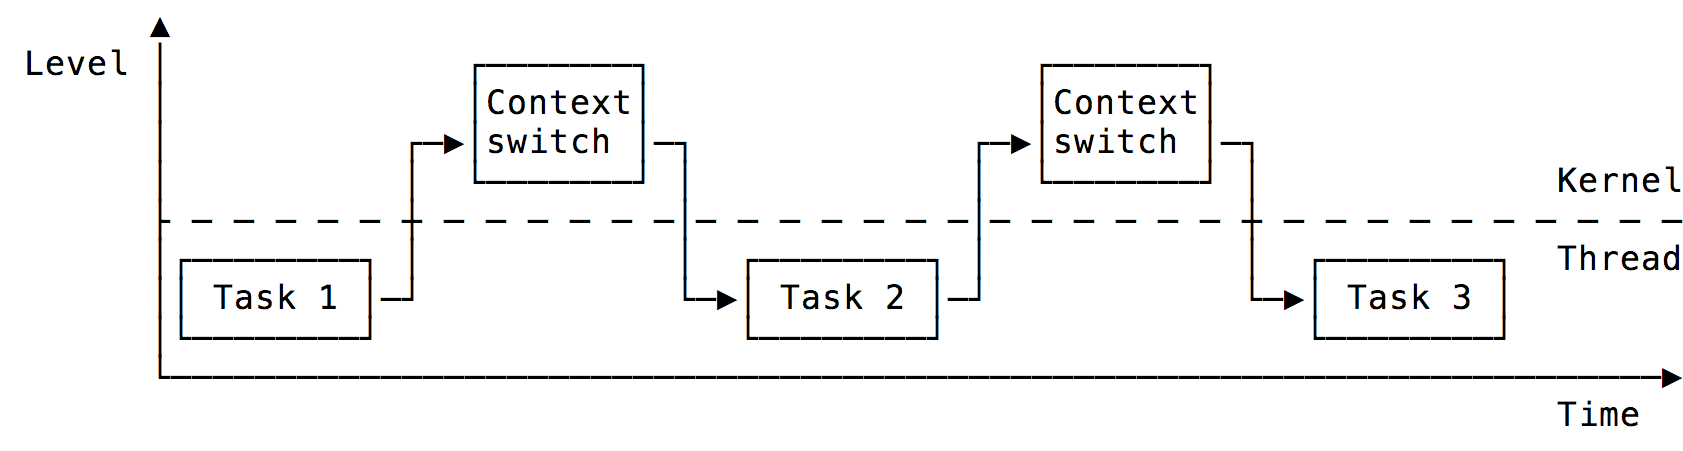
\includegraphics[width=0.9\textwidth]{contextswitch.png}
	\end{center}
	
\end{frame}


\begin{frame}
	\frametitle{Quando avviene un Context Switch}
	
	Il cambio di contesto può avvenire in diverse situazioni:
	
	\begin{itemize}
		
		\item scadenza del \textbf{quanto di tempo} nei sistemi time-sharing
		
		\item richiesta di \textbf{operazioni di I/O} da parte del processo
		
		\item arrivo di un \textbf{interrupt}
		
		\item terminazione di un processo
		
	\end{itemize}
	
	\textbf{Overhead}
	
	Il context switch introduce un costo computazionale
	perché la CPU deve:
	
	\begin{itemize}
		
		\item salvare e ripristinare registri e stato del processo
		\item aggiornare le strutture dati del sistema operativo
		\item eseguire codice del kernel
		
	\end{itemize}
	
	Durante queste operazioni la CPU non esegue lavoro utile
	per i programmi utente.
	
\end{frame}

	
% Sezione: Architettura e funzionamento di un sistema di calcolo

%------------------------------------------------

\begin{frame}
	\frametitle{Architettura di un sistema di calcolo}
	
	Un sistema di calcolo è composto da diversi componenti hardware
	che collaborano per eseguire i programmi.
	
	Componenti principali:
	
	\begin{itemize}
		\item \textbf{CPU (Central Processing Unit)}: esegue le istruzioni dei programmi.
		\item \textbf{Memoria principale (RAM)}: contiene dati e programmi in esecuzione.
		\item \textbf{Controller dei dispositivi}: componenti hardware che gestiscono le periferiche.
		\item \textbf{Bus di sistema}: canale di comunicazione tra CPU, memoria e dispositivi.
	\end{itemize}
	
	Il sistema operativo coordina l'utilizzo di queste componenti
	per garantire il corretto funzionamento del sistema.
	
\end{frame}

		 \begin{frame}
	\frametitle{Architettura di un sistema di calcolo}
	\begin{center}
		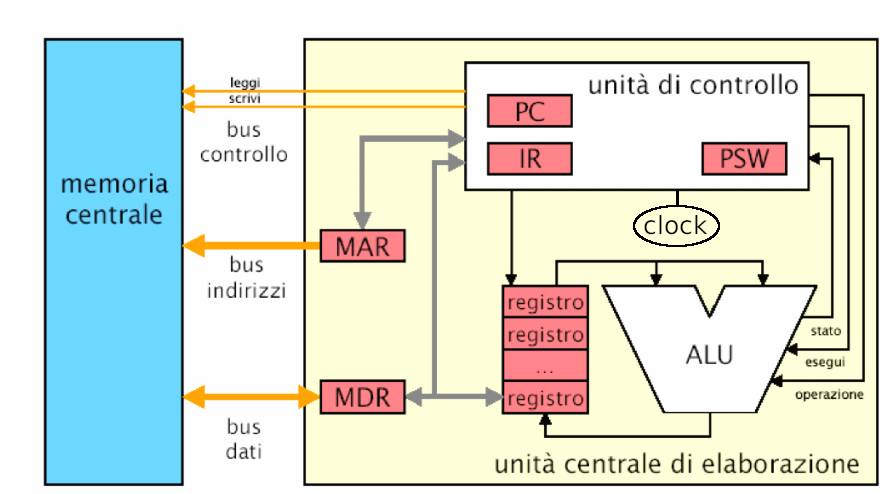
\includegraphics[width=0.9\textwidth]{architettura.png}
	\end{center}
	
\end{frame}

\begin{frame}
	\frametitle{Controller dei dispositivi}
	
	Le periferiche non comunicano direttamente con la CPU.
	
	Ogni dispositivo è gestito da un \textbf{controller}, cioè
	un componente hardware specializzato che controlla il dispositivo.
	
	Funzioni principali:
	
	\begin{itemize}
		\item ricevere comandi dalla CPU
		\item controllare il funzionamento del dispositivo
		\item trasferire dati tra dispositivo e memoria
	\end{itemize}
	
	Esempi:
	
	\begin{itemize}
		\item controller del disco
		\item controller video
		\item controller di rete
	\end{itemize}
	
\end{frame}

%------------------------------------------------

\begin{frame}
	\frametitle{Interrupt}
	
	Un \textbf{interrupt} è un segnale che interrompe temporaneamente
	l'esecuzione della CPU per segnalare il verificarsi di un evento.
	
	Gli \textbf{interrupt} permettono al sistema operativo di reagire
	rapidamente a eventi provenienti da hardware o software.
	
	Gli interrupt possono essere generati da:
	
	\begin{itemize}
		\item dispositivi hardware
		\item programmi in esecuzione
	\end{itemize}
	
\end{frame}

%------------------------------------------------

 \begin{frame}
	\frametitle{Interrupt}
	\begin{center}
		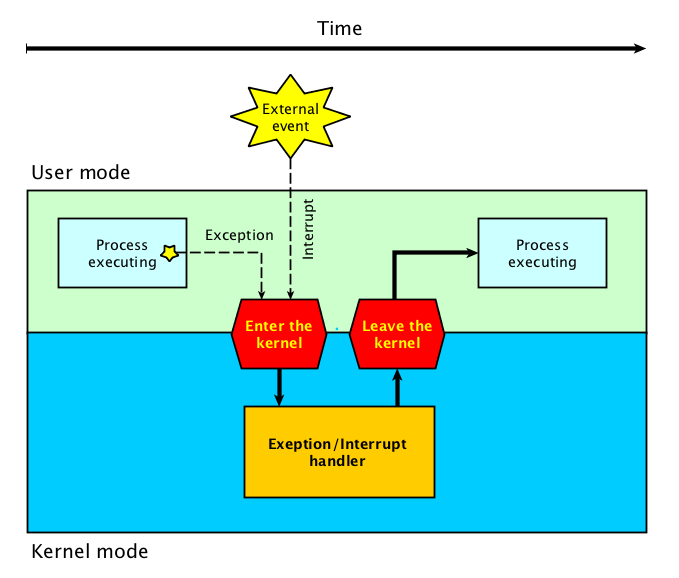
\includegraphics[width=0.6\textwidth]{interrupt_1.png}
	\end{center}
	\end{frame}

\begin{frame}
	\frametitle{Interrupt Hardware}
	
	Gli \textbf{interrupt hardware} sono generati dai dispositivi
	per segnalare eventi alla CPU.
	
	Esempi:
	
	\begin{itemize}
		\item completamento di una operazione di lettura da disco
		\item pressione di un tasto sulla tastiera
		\item arrivo di dati dalla rete
	\end{itemize}
	
	Quando avviene l'evento, il dispositivo invia un segnale
	alla CPU che interrompe temporaneamente il programma
	in esecuzione.
	
\end{frame}


 \begin{frame}
	\frametitle{Interrupt}
	\begin{center}
		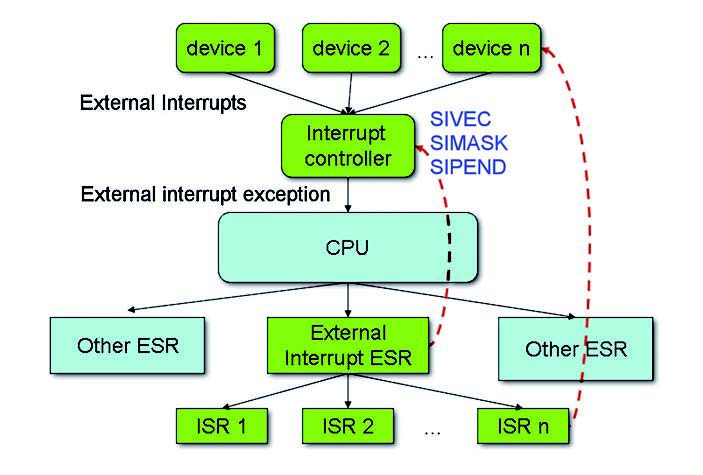
\includegraphics[width=0.6\textwidth]{interrupt_2.png}
	\end{center}
\end{frame}


%------------------------------------------------

\begin{frame}
	\frametitle{Interrupt Software}
	
	Gli \textbf{interrupt software} sono generati dai programmi
	in esecuzione.
	
	Possono essere causati da:
	
	\begin{itemize}
		\item errori durante l'esecuzione di un programma
		\item accessi illegali alla memoria
		\item richieste di servizi al sistema operativo
	\end{itemize}
	
	Un esempio importante di interrupt software è la
	\textbf{system call}, con cui un programma richiede
	un servizio al sistema operativo.
	
\end{frame}

%------------------------------------------------

\begin{frame}
	\frametitle{Gestione degli interrupt}
	
	Quando arriva un interrupt il sistema operativo esegue
	una sequenza di operazioni.
	
	\begin{enumerate}
		\item la CPU salva lo stato del processo corrente
		\item il controllo passa alla \textbf{routine di servizio dell'interrupt}
		\item viene gestito l'evento che ha generato l'interrupt
		\item lo stato del processo viene ripristinato
		\item il processo riprende l'esecuzione
	\end{enumerate}
	
	Questo meccanismo permette al sistema di reagire
	rapidamente agli eventi.
	
\end{frame}

%------------------------------------------------

\begin{frame}
	\frametitle{Input / Output}
	
	Le operazioni di \textbf{Input/Output (I/O)} permettono
	la comunicazione tra il computer e i dispositivi esterni.
	
	Esempi di dispositivi di I/O:
	
	\begin{itemize}
		\item tastiera
		\item disco
		\item stampante
		\item rete
	\end{itemize}
	
	Le operazioni di I/O sono generalmente più lente
	rispetto alle operazioni della CPU.
	
\end{frame}

%------------------------------------------------

\begin{frame}
	\frametitle{I/O sincrono}
	
	Nel caso di \textbf{I/O sincrono} il processo che richiede
	l'operazione rimane bloccato fino al completamento
	
	\begin{itemize}
		\item il processo non può proseguire
		\item la CPU può assegnare il tempo ad altri processi
	\end{itemize}
	
	Esempio:
	
	lettura di un file dal disco.
	
\end{frame}

%------------------------------------------------

\begin{frame}
	\frametitle{I/O asincrono}
	
	Nel caso di \textbf{I/O asincrono} il processo continua
	l'esecuzione mentre l'operazione di I/O viene svolta.
	
	Il completamento dell'operazione viene segnalato
	tramite un interrupt.
	
	Vantaggi:
	
	\begin{itemize}
		\item migliore utilizzo della CPU
		\item possibilità di eseguire più operazioni in parallelo
	\end{itemize}
	
\end{frame}

%------------------------------------------------

\begin{frame}
	\frametitle{DMA}
	
	\textbf{DMA (Direct Memory Access)} è una tecnica che
	permette ai dispositivi di trasferire dati direttamente
	tra dispositivo e memoria.
	
	Senza DMA:
	
	\begin{itemize}
		\item la CPU deve gestire ogni trasferimento di dati
	\end{itemize}
	
	Con DMA:
	
	\begin{itemize}
		\item il trasferimento avviene senza coinvolgere la CPU
		\item la CPU può eseguire altre operazioni
	\end{itemize}
	
	Vantaggi:
	
	\begin{itemize}
		\item minore carico sulla CPU
		\item maggiore velocità nei trasferimenti
	\end{itemize}
	
\end{frame}

 \begin{frame}
	\frametitle{Direct Memory Access}
	\begin{center}
		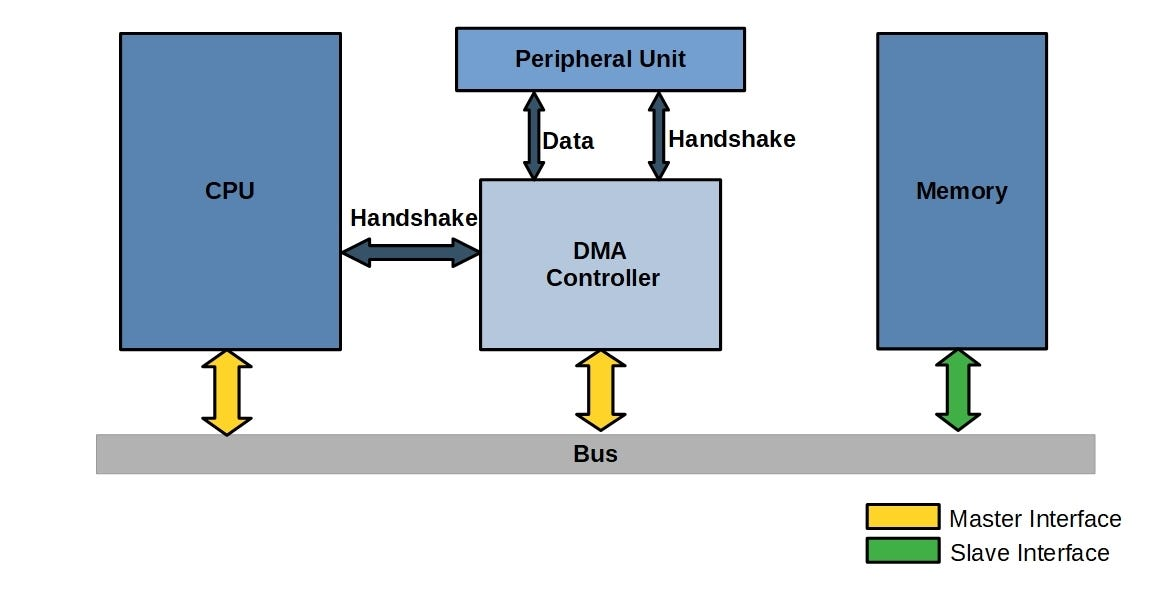
\includegraphics[width=0.6\textwidth]{dma.jpg}
	\end{center}
\end{frame}

%------------------------------------------------

\begin{frame}
	\frametitle{Protezione del sistema}
	
	Nei sistemi multiprogrammati o multiutente
	è necessario proteggere le risorse del sistema.
	
	Le principali risorse da proteggere sono:
	
	\begin{itemize}
		\item memoria
		\item processi
		\item file
		\item dispositivi
	\end{itemize}
	
	Il sistema operativo impedisce che un programma
	interferisca con il funzionamento degli altri.
	
\end{frame}

%------------------------------------------------

\begin{frame}
	\frametitle{Dual Mode}
	
	Molte architetture hardware prevedono due modalità
	di esecuzione.
	
	\begin{itemize}
		\item \textbf{User Mode}: esecuzione dei programmi utente
		\item \textbf{Kernel Mode}: esecuzione del sistema operativo
	\end{itemize}
	
	Solo il kernel può eseguire \textbf{istruzioni privilegiate}
	come l'accesso ai dispositivi o la gestione della memoria.
	
	Questo meccanismo aumenta la sicurezza del sistema.
	
\end{frame}

%------------------------------------------------

\begin{frame}
	\frametitle{System Call}
	
	Le \textbf{system call} sono l'interfaccia tra
	programmi utente e sistema operativo.
	
	Permettono ai programmi di richiedere servizi
	al kernel.
	
	Esempi di system call:
	
	\begin{itemize}
		\item open()
		\item read()
		\item write()
		\item fork()
	\end{itemize}
	
\end{frame}

%------------------------------------------------

\begin{frame}[fragile]
	\frametitle{Esempio Linux}
	
	Esempio di system call:
	
	\begin{verbatim}
		read(fd, buffer, size);
	\end{verbatim}
	
	Il programma richiede al kernel di leggere dati
	associati al file descriptor \texttt{fd} e salvarli
	nel buffer di memoria.
	
\end{frame}

%------------------------------------------------

\begin{frame}
	\frametitle{Processo}
	
	Un \textbf{processo} è un programma in esecuzione.
	
	Oltre al codice del programma include:
	
	\begin{itemize}
		\item dati del programma
		\item registri della CPU
		\item contatore di programma
		\item informazioni sullo stato di esecuzione
	\end{itemize}
	
	Il processo rappresenta l'unità fondamentale
	di esecuzione nel sistema operativo.
	
\end{frame}

%------------------------------------------------

\begin{frame}
	\frametitle{Gestione dei processi}
	
	Il sistema operativo gestisce l'intero ciclo
	di vita dei processi.
	
	Compiti principali:
	
	\begin{itemize}
		\item creazione dei processi
		\item terminazione dei processi
		\item sospensione e ripresa dei processi
		\item sincronizzazione tra processi
	\end{itemize}
	
	Queste operazioni sono gestite tramite
	strutture dati interne al sistema operativo.
	
\end{frame}


 \begin{frame}
	\frametitle{Gestione dei processi}
	\begin{center}
		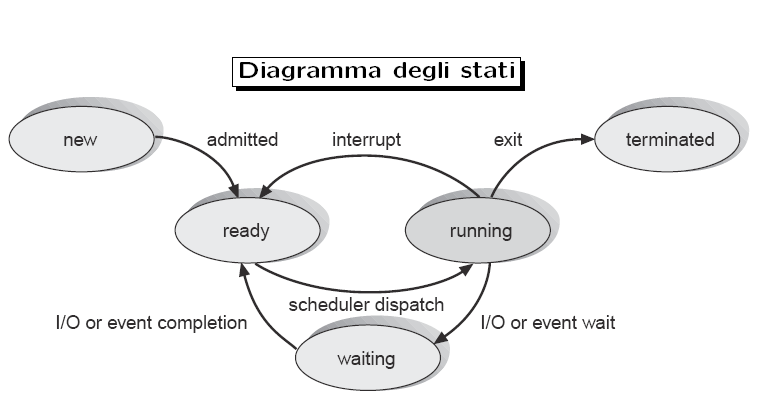
\includegraphics[width=0.6\textwidth]{gestioneprocessi.png}
	\end{center}
\end{frame}


%------------------------------------------------

\begin{frame}
	\frametitle{Gestione della memoria}
	
	La \textbf{memoria principale} è una risorsa limitata
	che deve essere condivisa tra più processi.
	
	Il sistema operativo deve:
	
	\begin{itemize}
		\item allocare memoria ai processi
		\item liberare memoria quando non serve più
		\item proteggere gli spazi di memoria
	\end{itemize}
	
\end{frame}


 \begin{frame}
	\frametitle{Gestione della memoria}
	\begin{center}
		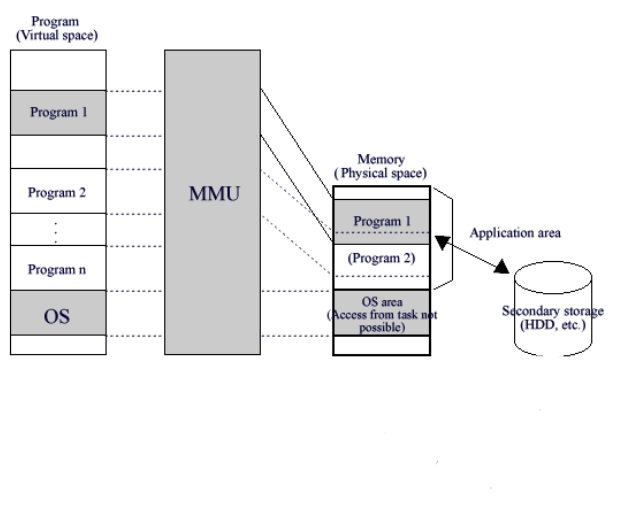
\includegraphics[width=0.6\textwidth]{gestionememoria.png}
	\end{center}
\end{frame}




%------------------------------------------------

\begin{frame}
	\frametitle{Memoria Virtuale}
	
	La \textbf{memoria virtuale} permette di utilizzare
	uno spazio di memoria logico più grande
	della memoria fisica disponibile.
	
	Il sistema operativo utilizza il disco
	come estensione della memoria.
	
	Vantaggi:
	
	\begin{itemize}
		\item esecuzione di programmi di grandi dimensioni
		\item migliore gestione della memoria
	\end{itemize}
	
\end{frame}

%------------------------------------------------

\begin{frame}
	\frametitle{Gestione dei File}
	
	Il sistema operativo fornisce una visione
	astratta della memoria secondaria tramite
	il concetto di \textbf{file}.
	
	Funzioni principali:
	
	\begin{itemize}
		\item creazione e cancellazione dei file
		\item organizzazione in directory
		\item gestione dei permessi di accesso
	\end{itemize}
	
\end{frame}

%------------------------------------------------

\begin{frame}
	\frametitle{File System}
	
	Il \textbf{file system} definisce come i dati
	sono organizzati e memorizzati sui dispositivi.
	
	Esempi di file system:
	
	\begin{itemize}
		\item NTFS
		\item ext4
		\item FAT32
		\item APFS
	\end{itemize}
	
	Ogni sistema operativo supporta uno o più
	file system.
	
\end{frame}

%------------------------------------------------

\begin{frame}
	\frametitle{Gestione I/O}
	
	Il sistema operativo gestisce le operazioni
	di input/output tramite diversi meccanismi.
	
	\begin{itemize}
		\item driver di dispositivo
		\item buffer per memorizzazione temporanea
		\item code di richieste
	\end{itemize}
	
	Questi strumenti permettono di gestire
	più richieste contemporaneamente.
	
\end{frame}

%------------------------------------------------

\begin{frame}
	\frametitle{Driver di dispositivo}
	
	Un \textbf{driver} è un software che permette
	al sistema operativo di comunicare con
	un dispositivo hardware.
	
	Esempi:
	
	\begin{itemize}
		\item driver stampante
		\item driver scheda video
		\item driver scheda di rete
	\end{itemize}
	
	I driver nascondono i dettagli specifici
	dell'hardware.
	
\end{frame}

%------------------------------------------------

\begin{frame}
	\frametitle{Sicurezza}
	
	La sicurezza del sistema operativo serve
	a proteggere il sistema e i dati.
	
	Minacce principali:
	
	\begin{itemize}
		\item accessi non autorizzati
		\item attacchi di rete
		\item malware
	\end{itemize}
	
	Il sistema operativo utilizza meccanismi
	di autenticazione e controllo degli accessi.
	
\end{frame}

%------------------------------------------------

\begin{frame}
	\frametitle{Interfaccia utente}
	
	L'interfaccia utente permette agli utenti
	di interagire con il sistema operativo.
	
	Due tipi principali:
	
	\begin{itemize}
		\item \textbf{CLI} (Command Line Interface)
		\item \textbf{GUI} (Graphical User Interface)
	\end{itemize}
	
\end{frame}

%------------------------------------------------

\begin{frame}[fragile]
	\frametitle{CLI}
	
	La CLI permette di interagire con il sistema
	tramite comandi testuali.
	
	Esempio Linux:
	
	\begin{verbatim}
		ls
		cd
		mkdir
	\end{verbatim}
	
\end{frame}


 \begin{frame}
	\frametitle{Command Line Interface}
	\begin{center}
		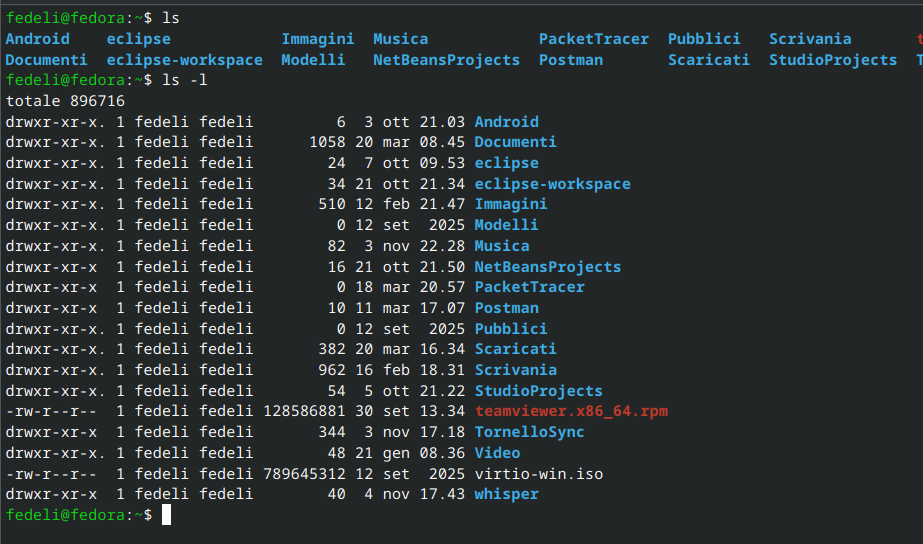
\includegraphics[width=0.6\textwidth]{cli.png}
	\end{center}
\end{frame}


%------------------------------------------------

\begin{frame}
	\frametitle{GUI}
	
	La GUI permette di interagire con il sistema
	tramite elementi grafici.
	
	\begin{itemize}
		\item finestre
		\item icone
		\item menu
		\item mouse
	\end{itemize}
	
\end{frame}

%------------------------------------------------

\begin{frame}
	\frametitle{Componenti di un Sistema Operativo}
	
	Principali moduli del sistema operativo:
	
	\begin{itemize}
		\item gestione dei processi
		\item gestione della memoria
		\item gestione dei file
		\item gestione dell'I/O
		\item sicurezza
	\end{itemize}
	
\end{frame}

%------------------------------------------------

\begin{frame}
	\frametitle{Struttura Monolitica}
	
	In una struttura monolitica
	il sistema operativo è un unico grande programma.
	
	Esempi storici:
	
	\begin{itemize}
		\item MS-DOS
		\item prime versioni di UNIX
	\end{itemize}
	
\end{frame}


\begin{frame}
	\frametitle{Struttura Monolitica}
	
	In una struttura monolitica il sistema operativo è
	un unico grande programma eseguito in modalità kernel.
	
	\vspace{0.3cm}
	
	\textbf{Caratteristiche}
	\begin{itemize}
		\item Tutti i servizi (file system, memoria, I/O, driver) sono nello stesso spazio
		\item Comunicazione diretta tra componenti (chiamate di funzione)
		\item Elevate prestazioni (basso overhead)
	\end{itemize}
	
	\vspace{0.3cm}
	
	\textbf{Svantaggi}
	\begin{itemize}
		\item Scarsa modularità
		\item Difficile manutenzione ed estensione
		\item Un errore può compromettere tutto il sistema
	\end{itemize}
	
	\vspace{0.3cm}
	
	\textbf{Esempi}
	\begin{itemize}
		\item MS-DOS
		\item prime versioni di UNIX
	\end{itemize}
	
\end{frame}

%------------------------------------------------

\begin{frame}
	\frametitle{Struttura a livelli}
	
	In una struttura a livelli
	il sistema operativo è organizzato
	in livelli gerarchici.
	
	Ogni livello utilizza i servizi
	del livello sottostante.
	
\end{frame}


\begin{frame}
	\frametitle{Struttura a livelli}
	
	In una struttura a livelli il sistema operativo è suddiviso
	in livelli gerarchici, ciascuno con una funzione specifica.
	
	\vspace{0.3cm}
	
	\textbf{Principio}
	\begin{itemize}
		\item Ogni livello utilizza solo i servizi del livello sottostante
		\item Fornisce servizi al livello superiore
		\item Nasconde i dettagli implementativi (astrazione)
	\end{itemize}
	
	\vspace{0.3cm}
	
	\textbf{Esempio di livelli}
	\begin{itemize}
		\item Hardware
		\item Gestione memoria
		\item Gestione processi
		\item File system
		\item Interfaccia utente
	\end{itemize}
	
	\vspace{0.3cm}
	
	\textbf{Vantaggi e svantaggi}
	\begin{itemize}
		\item Maggiore modularità e facilità di manutenzione
		\item Migliore isolamento tra componenti
		\item Possibile perdita di prestazioni (passaggi tra livelli)
	\end{itemize}
	
\end{frame}

%------------------------------------------------
 \begin{frame}
	\frametitle{Struttura a livelli}
	\begin{center}
		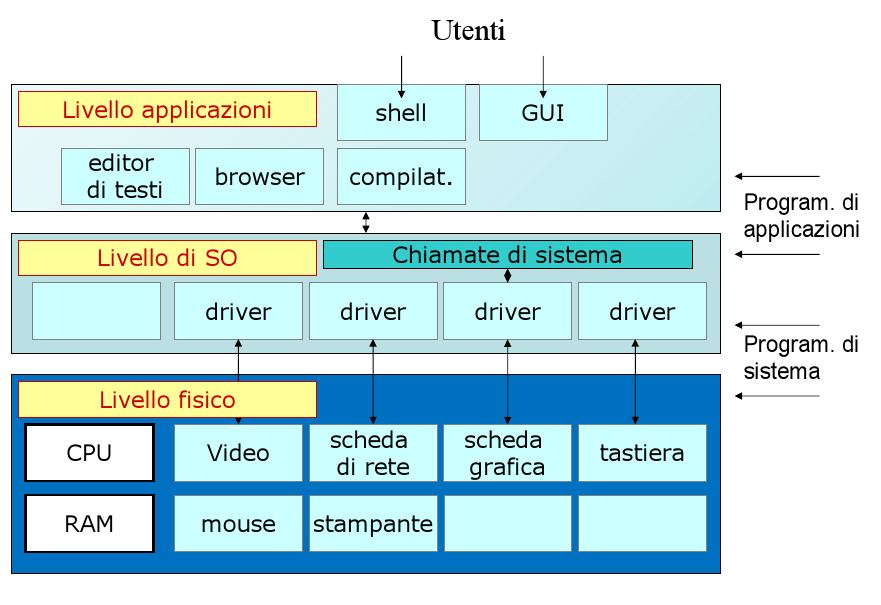
\includegraphics[width=0.8\textwidth]{strutturalivelli.png}
	\end{center}
\end{frame}

%------------------------------------------------

\begin{frame}
	\frametitle{Kernel}
	
	Il \textbf{kernel} è il nucleo del sistema operativo.
	
	Gestisce le operazioni fondamentali:
	
	\begin{itemize}
		\item gestione dei processi
		\item gestione della memoria
		\item gestione degli interrupt
		\item gestione delle system call
	\end{itemize}
	
\end{frame}

%------------------------------------------------

\begin{frame}
	\frametitle{Microkernel}
	
	Nel modello microkernel il kernel contiene
	solo le funzionalità minime indispensabili.
	
	\vspace{0.3cm}
	
	\textbf{Funzioni nel kernel}
	\begin{itemize}
		\item Gestione dei processi (scheduling)
		\item Gestione della memoria di base
		\item Comunicazione tra processi (IPC)
	\end{itemize}
	
	\vspace{0.3cm}
	
	\textbf{Servizi esterni al kernel}
	\begin{itemize}
		\item File system
		\item Driver di dispositivo
		\item Gestione rete
	\end{itemize}
	
	\vspace{0.3cm}
	
	\textbf{Caratteristiche}
	\begin{itemize}
		\item Comunicazione tramite messaggi (IPC)
		\item Elevato isolamento tra componenti
	\end{itemize}
	
	\vspace{0.3cm}

	
\end{frame}

%------------------------------------------------

\begin{frame}
	\frametitle{Vantaggi del Microkernel}
	
		
	\textbf{Vantaggi e svantaggi}
	\begin{itemize}
		\item Maggiore sicurezza e stabilità
		\item Più facile manutenzione
		\item Possibile overhead nelle comunicazioni
	\end{itemize}

\end{frame}

%------------------------------------------------

\begin{frame}
	\frametitle{Svantaggi del Microkernel}
	
	\begin{itemize}
		\item maggiore comunicazione tra processi
		\item possibile riduzione delle prestazioni
	\end{itemize}
	
\end{frame}


%------------------------------------------------

\begin{frame}
	\frametitle{Conclusioni}
	
	Il sistema operativo è il componente
	fondamentale di ogni computer.
	
	Permette di:
	
	\begin{itemize}
		\item gestire le risorse hardware
		\item eseguire applicazioni
		\item garantire sicurezza e stabilità
	\end{itemize}
	
\end{frame}
	
	%------------------------------------------------
	
\begin{frame}
	\frametitle{Riferimenti Bibliografici}
	
	\begin{thebibliography}{10}
		
		\bibitem{silberschatz}
		A. Silberschatz, P. B. Galvin, G. Gagne \\
		\textit{Operating System Concepts} \\
		Wiley, ultima edizione.
		
		\bibitem{tanenbaum}
		A. S. Tanenbaum, H. Bos \\
		\textit{Modern Operating Systems} \\
		Pearson.
		
		\bibitem{stallings}
		W. Stallings \\
		\textit{Operating Systems: Internals and Design Principles} \\
		Pearson.
		
		\bibitem{love}
		R. Love \\
		\textit{Linux Kernel Development} \\
		Addison-Wesley.
		
		\bibitem{ciampolini}
		A. Ciampolini \\
		\textit{Sistemi Operativi -- Materiale didattico} \\
		Università di Bologna.
		
	\end{thebibliography}
	
\end{frame}
	
\end{document}
